\documentclass[tikz,border=2pt]{standalone}
\usepackage{amsmath}
\usetikzlibrary{arrows.meta}
\begin{document}
% seq(0, 1, by = 0.3) = 0, 0.3, 0.6, 0.9 (the next value 1.2 passes to = 1);
% seq(0, 5, length.out = 5) = 0, 1.25, 2.5, 3.75, 5 (step (5 - 0)/4 = 1.25).
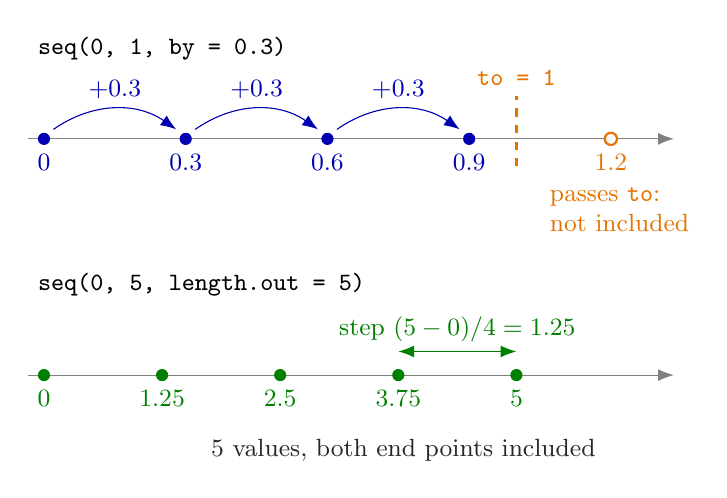
\begin{tikzpicture}[font=\small, >={Latex[length=2mm]}]
  % ---------- by = 0.3 (unit: 6 cm) ----------
  \begin{scope}
    \node[anchor=west, font=\small\ttfamily] at (-0.2,1.15) {seq(0, 1, by = 0.3)};
    \draw[gray, ->] (-0.2,0) -- (8.0,0);
    \foreach \v/\l in {0/0, 0.3/0.3, 0.6/0.6, 0.9/0.9} {
      \fill[blue!70!black] (6*\v,0) circle (2.2pt);
      \node[below=2pt, blue!70!black] at (6*\v,0) {$\l$};
    }
    \foreach \a in {0,0.3,0.6} {
      \draw[blue!70!black, ->, bend left=35] (6*\a+0.12,0.12) to node[above, font=\small] {$+0.3$} (6*\a+1.68,0.12);
    }
    \draw[orange!90!black, dashed, thick] (6,-0.35) -- (6,0.55);
    \node[orange!90!black, above] at (6,0.55) {\texttt{to = 1}};
    \draw[orange!90!black, thick, fill=white] (7.2,0) circle (2.2pt);
    \node[orange!90!black, below=2pt] at (7.2,0) {$1.2$};
    \node[orange!90!black, anchor=west, align=left] at (6.3,-0.9) {passes \texttt{to}:\\ not included};
  \end{scope}
  % ---------- length.out = 5 (unit: 1.2 cm) ----------
  \begin{scope}[yshift=-3.0cm]
    \node[anchor=west, font=\small\ttfamily] at (-0.2,1.15) {seq(0, 5, length.out = 5)};
    \draw[gray, ->] (-0.2,0) -- (8.0,0);
    \foreach \v/\l in {0/0, 1.25/1.25, 2.5/2.5, 3.75/3.75, 5/5} {
      \fill[green!50!black] (1.2*\v,0) circle (2.2pt);
      \node[below=2pt, green!50!black] at (1.2*\v,0) {$\l$};
    }
    \draw[green!50!black, <->] (4.5,0.3) -- node[above] {step $(5-0)/4=1.25$} (6.0,0.3);
    \node[gray!30!black, anchor=west] at (2.0,-0.95) {5 values, both end points included};
  \end{scope}
\end{tikzpicture}
\end{document}
